% Name: Skip list
% Description: A skip list of six keys on four levels, each key promoted to a random height, with the search for 25 in orange dropping down a level whenever the next key is too large.
% Tags: skip list, linked list, search, randomized data structure

\usetikzlibrary{arrows.meta}

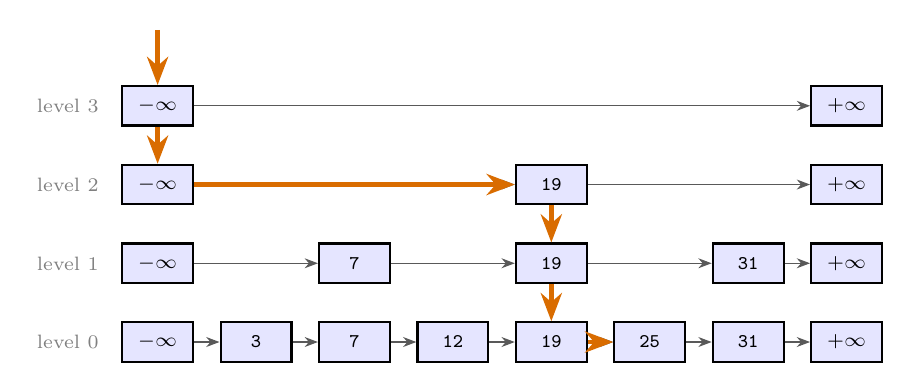
\begin{tikzpicture}[>={Stealth}, x=1.25cm, y=1cm,
    cell/.style={draw, thick, fill=blue!10, minimum width=9mm, minimum height=5mm, inner sep=0pt, font=\scriptsize\ttfamily}]
  % Column i holds key k with height h; the sentinels are full height
  \foreach \i/\k/\h in {0/{$-\infty$}/4, 1/3/1, 2/7/2, 3/12/1, 4/19/3, 5/25/1, 6/31/2, 7/{$+\infty$}/4}
    \foreach \l in {1,...,\h} \node[cell] (c\i-\l) at (\i,\l-1) {\k};
  % Each level links every tower tall enough to reach it
  \foreach \l/\list in {1/{0,1,2,3,4,5,6,7}, 2/{0,2,4,6,7}, 3/{0,4,7}, 4/{0,7}} {
    \def\prev{}
    \foreach \i in \list {
      \ifx\prev\empty\else \draw[->, gray!70!black] (c\prev-\l) -- (c\i-\l); \fi
      \xdef\prev{\i}
    }
  }
  % Level 3 reaches +inf at once, so the search drops to level 2, moves to 19, then drops twice before 25 is next
  \draw[->, line width=1.6pt, orange!85!black] (c0-4.north) ++(0,0.7) -- (c0-4.north);
  \draw[line width=1.6pt, orange!85!black, ->] (c0-4) -- (c0-3);
  \draw[line width=1.6pt, orange!85!black, ->] (c0-3) -- (c4-3);
  \draw[line width=1.6pt, orange!85!black, ->] (c4-3) -- (c4-2);
  \draw[line width=1.6pt, orange!85!black, ->] (c4-2) -- (c4-1);
  \draw[line width=1.6pt, orange!85!black, ->] (c4-1) -- (c5-1);
  \foreach \l in {1,...,4} \node[font=\scriptsize, gray, anchor=east] at (-0.5,\l-1) {level \the\numexpr\l-1\relax};
\end{tikzpicture}
